\section{Udviklingsforløb}
I dette afsnit vil metoderne, der er blevet brugt i projektet, blive forklaret, hvordan disse er blevet benyttet og deres bidrag til projektet.

\subsection{ASE-modellen} \label{sec:ASEModel}
Den udviklingsmodel, som primært er brugt i projektet, er ASE modellen, som ses på figur \ref{fig:ASE}. ASE modellen \cite{ASE} er en mellemvægtig semi-iterativ udviklingsmodel, som er drevet ud fra en kravspecifikation, der bygger på user stories. ASE modellen tager udgangspunkt i vandfaldsmodellen til at opbygge dit projekt gennem faserne: Projektformulering - Kravspecifikation - Systemarkitektur -  Implementering -  Test/fejlfinding -  Integration og vedligeholdelse\cite{ASE}.

\begin{figure} [H]
	\begin{center}
		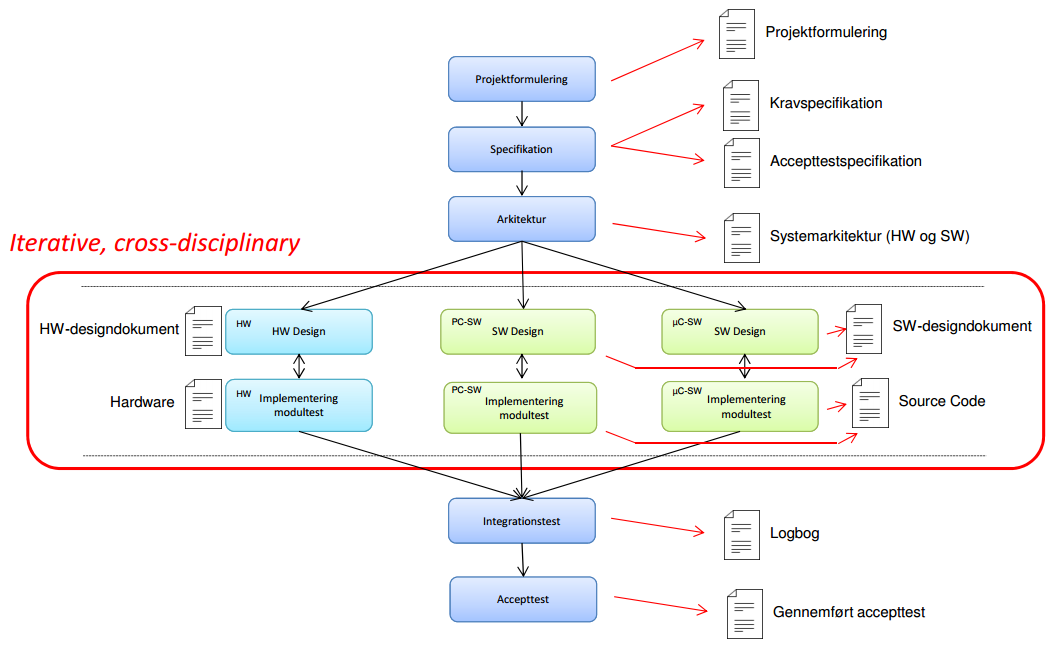
\includegraphics[height=10cm, width=12cm]{Udviklingsforlob/ASEModellen}
	\end{center}
	\caption{ASE modellen. \cite{ASE}}
	\label{fig:ASE}
\end{figure}

Første punkt i ASE modellen er, at få skrevet en projektformulering og herefter en kravspecifikation, som består af en række user stories. User stories er et værktøj, der beskriver, hvordan der interageres med systemet. Efterfølgende opbygges en kravspecifikation ud fra user stories, og herved opnås et godt overblik over, hvilke krav der er til systemet. Accepttesten specificeres derefter ud fra kravspecifikationen, så alle dele i det samlede system bliver testet.
Der er tilføjet en analyse til modellen for at kunne redegøre for de valg, der er taget i projektet. Analysen blev udarbejdet sideløbende med kravspecifikationen. \\
Når kravspecifikationen er udarbejdet, påbegyndes udarbejdningen af systemarkitekturen. I systemarkitekturen skematiseres systemets moduler og grænseflader til de andre moduler i systemet. Når den overordnede arkitektur er på plads, brydes systemet op efter funktionalitet. \\
I design- og implementeringsfaserne er der anvendt en iterativ proces. Dette har gjort udviklingen mere fleksibel. \\

\subsection{Kanban}
Kanban \cite{Kanban} er en agil udviklingsproces med fokus på projektledelse. Forskellen på Kanban og andre arbejdsmetoder som f.eks. vandfaldmodellen\cite{Vandfald} er, at Kanban er en iterativ proces og ikke en lineær proces.

Til visualisering af arbejdsopgaverne i Kanban, bruges et Kanban-board. Her har udviklingsteamet mulighed for at få overblik over opgaver og standardisere gruppens workflow. Der er typisk 3 steps på et Kanban board: To Do, Doing, Done. Der kan tilføjes et fjerde step: Review. \\
\emph{To Do} er alle opgaver som skal laves. \\
\emph{Doing} er opgaver som team'et pt arbejder på. \\
\emph{Done} er alle opgaver, der er færdige. \\
\emph{Review} er opgaver som er færdige, men som et andet medlem af team'et skal gennemgå og godkende før det kan flyttes i Done.\\
Et standard kanban board kan se ud som på figur \ref{fig:Kanban}.
\begin{figure} [H]
	\begin{center}
		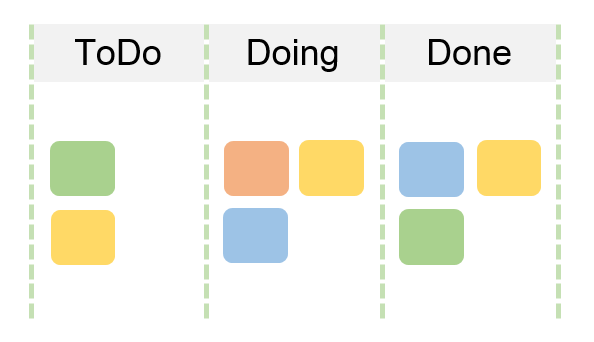
\includegraphics[height=5cm, width=10cm]{Udviklingsforlob/kanbanboard}
	\end{center}
	\caption{Et standard Kanban board. \cite{Kanban}}
	\label{fig:Kanban}
\end{figure}

Fordele ved Kanban er en fleksibel agil udviklingsproces, hvor at man nemt kan omrokere opgaver, hvis der sker en ændring i prioriteringen af hvad der skal laves først. \\
Derudover giver Kanban en masse frihed i forhold til flowet, da det er kontinuerligt gennem hele projektet. Der kan også løbende laves ændringer i team'et hvis dette er nødvendigt. \\



